\documentclass{beamer}

\usepackage{listings}
\usepackage{tabularx}
\usepackage{booktabs}
\usepackage{makecell}
\usepackage{siunitx}
\usepackage{color}


\lstset{frame=tb,
  language=Java,
  aboveskip=3mm,
  belowskip=3mm,
  showstringspaces=false,
  columns=flexible,
  basicstyle={\small\ttfamily},
  numbers=none,
  numberstyle=\tiny\color{gray},
  keywordstyle=\color{blue},
  commentstyle=\color{gray},
  stringstyle=\color{red},
  breaklines=true,
  breakatwhitespace=true,
  tabsize=3
}

\usetheme{focus}
\definecolor{background}{RGB}{255, 255, 255}
\setbeamerfont{title}{size=\LARGE}
\setbeamerfont{author}{size=\large}
\setbeamertemplate{itemize item}{\textbullet}

%Information to be included in the title page:
\title{
    Considerations for integrating virtual threads in a Java framework: a Quarkus example in a resource-constrained environment}
\author[Navarro, Ponge, Le Mouël, Escoffier]{A.~Navarro\inst{1,2} \and J.~Ponge\inst{1,2}\and F.~Le~Mouël\inst{2}\and C.~Escoffier\inst{1}}
\institute{\inst{1}Red Hat  ~\inst{2}CITI Laboratory-INSA Lyon}
\date{2023}

% \setbeamertemplate{sidebar right}{}
% \setbeamertemplate{footline}{%
% \hfill\usebeamertemplate***{navigation symbols}
% \hspace{1cm}\insertframenumber{}/\inserttotalframenumber}

\begin{document}

\frame{\titlepage}

\AtBeginSection[]
{
  \begin{frame}
    \frametitle{Table of Contents}
    \tableofcontents[currentsection]
  \end{frame}
}


\section{Context}
\begin{frame}{The end of the monolith}
    \begin{columns}
        \begin{column}{0.5\textwidth}
            \begin{itemize}
                \item difficult to maintain
                \item dependency hell
                \item reboot for every change
            \end{itemize}
        \end{column}
        \begin{column}{0.5\textwidth}
            \begin{itemize}
                \item sub-optimal deployment
                \item limit scalability
                \item technology lock-in
            \end{itemize}
        \end{column}
    \end{columns}
    \vspace{1cm}
    \begin{block}{from}
        Microservices: yesterday, today, and tomorrow - Dragoni \& al
    \end{block}
\end{frame}
\begin{frame}{Microservices}
    \begin{columns}
        \begin{column}{0.53\textwidth}
            \begin{itemize}
                \item \emph{\textcolor{red}{difficult to maintain}}
                \item split in smaller entities 
                \item \emph{\textcolor{red}{dependency hell}}
                \item less dependencies per service
                \item \emph{\textcolor{red}{reboot for every change}}
                \item reboot only impacted service
            \end{itemize}
        \end{column}
        \begin{column}{0.5\textwidth}
            \begin{itemize}
                \item \emph{\textcolor{red}{sub-optimal deployment}}
                \item per-service deployment
                \item \emph{\textcolor{red}{limits scalability}}
                \item scale each service
                \item \emph{\textcolor{red}{technology lock-in}}
                \item per service technology
            \end{itemize}
        \end{column}
    \end{columns}
    \vspace{1cm}
    \begin{alertblock}{Remark}
        Transitioning to cloud becomes a thing
    \end{alertblock}
\end{frame}
\begin{frame}{Make microservices cheap}
    \setbeamertemplate{itemize item}{}
    \begin{columns}
        \begin{column}{0.36\textwidth}
            \begin{itemize}
                \item resource-efficiency
                \item resource-efficiency
                \item resource-efficiency
                \item resource-efficiency
                \item resource-efficiency
                \item resource-efficiency
                \item resource-efficiency
                \item resource-efficiency
                \item resource-efficiency
                \item resource-efficiency
                \item resource-efficiency
                \item resource-efficiency
                \item resource-efficiency
                \item resource-efficiency
                \item resource-efficiency
            \end{itemize}
        \end{column}
        \begin{column}{0.36\textwidth}
            \begin{itemize}
                \item resource-efficiency
                \item resource-efficiency
                \item resource-efficiency
                \item resource-efficiency
                \item resource-efficiency
                \item resource-efficiency
                \item resource-efficiency
                \item resource-efficiency
                \item resource-efficiency
                \item resource-efficiency
                \item resource-efficiency
                \item resource-efficiency
                \item resource-efficiency
                \item resource-efficiency
                \item resource-efficiency
            \end{itemize}
        \end{column}
        \begin{column}{0.36\textwidth}
            \begin{itemize}
                \item resource-efficiency
                \item resource-efficiency
                \item resource-efficiency
                \item resource-efficiency
                \item resource-efficiency
                \item resource-efficiency
                \item resource-efficiency
                \item resource-efficiency
                \item resource-efficiency
                \item resource-efficiency
                \item resource-efficiency
                \item resource-efficiency
                \item resource-efficiency
                \item resource-efficiency
                \item resource-efficiency
            \end{itemize}
        \end{column}
    \end{columns}
\end{frame}
\begin{frame}{Scaling and reactive programming}
    \begin{alertblock}{Problem}
        communications over the network are unreliable and slow
    \end{alertblock}
    \begin{block}{Solutions}
        efficient and timely communication between services
        historically brought by non-blocking, asynchronous abstractions in the OS
    \end{block}
\end{frame}
\begin{frame}{Non-blocking abstractions}
    \begin{columns}
        \begin{column}{0.5\textwidth}
            \begin{itemize}
                \item asynchronous callbacks
                \item promises and futures
                \item reactive streams
            \end{itemize}
        \end{column}
        \begin{column}{0.5\textwidth}
            \begin{itemize}
                \item coroutines
                \item async functions
                \item light threads
            \end{itemize}
        \end{column}
    \end{columns}
\end{frame}
\begin{frame}{Finally, virtual threads}
    \includegraphics[width=\textwidth]{assets/threads_virtual_threads.png}
\end{frame}
\begin{frame}[fragile]{Code comparison - blocking}
    \begin{figure}
        \begin{lstlisting}
var names = getAll();
var quotes = getQuotes(names.size());
for(int i=0; i < names.size();i ++){
    names.get(i).surname+= ” - ”+quotes.get(i);
}
return names;
        \end{lstlisting}
    \end{figure}
\end{frame}
\begin{frame}[fragile]{Code comparison - asynchronous callbacks}
    \begin{figure}
        \begin{lstlisting}
getAll( names => {
    getQuotes(names.size(), quotes => {
        for(int i=0; i < names.size();i ++){
            names.get(i).surname+= ” - ”+quotes.get(i);
        }
        //continuation
    })
});
        \end{lstlisting}
    \end{figure}
\end{frame}
\begin{frame}[fragile]{Code comparison - reactive streams}
    \begin{figure}
        \begin{lstlisting}
var names = getAll().memoize().indefinitely();
var quotes = names.onItem().transformToUni(list -> 
            getQuotes(list.size()));
return Uni.combine().all()
    .unis(names,quotes).asTuple()
    .onItem().transform(tuple -> {
        var nList=tuple.getItem1();
        //can await it since it is already resolved
        var qList = tuple.getItem2();
        for(int i=0; i  < namesList.size();i ++){
            nList.get(i).surname += "   -  "+qList.get(i);
        }
        return namesList;
    });
        \end{lstlisting}
    \end{figure}
\end{frame}
\begin{frame}[fragile]{Code comparison - virtual threads}
    \begin{figure}
        \begin{lstlisting}
var names = getAll();
var quotes = getQuotes(names.size());
for(int i=0; i < names.size();i ++){
    names.get(i).surname+= ” - ”+quotes.get(i);
}
return names;
        \end{lstlisting}
    \end{figure}
\end{frame}
\begin{frame}{Asynchronous programming abstractions}
    \begin{quote}
        We should do (as wise programmers aware of our limitations) our utmost best to shorten the conceptual gap between the static program and the dynamic process, to \textbf{make the correspondence between the program (spread out in text space) and the process (spread out in time) as trivial as possible}.
    \end{quote}
    Edgar. J. Dijkstra, 1968
\end{frame}

\section{Integration}
\begin{frame}{Three integration strategies}
    \begin{table}[htb]
    \centering
    \setlength{\tabcolsep}{2pt}
    \small
    \begin{tabularx}{\columnwidth}{ @{}| X || X | X |@{}}
        \hline
        \thead{Strategy} &  \thead{Pros}
        &   \thead{Cons} \\
        \hline\hline
        Forking worker model & Simple, fits virtual threads model & Context switches\\
        \hline
        Using event-loop as carrier & No context-switch, Fewer threads overall 
        & Potential deadlocks \\
        \hline
        Modifying Netty event-loops to be virtual threads 
        & Integration done at the Netty level, Netty-based frameworks would benefit from it
        & Can't modify Netty upstream, unpredictable effects\\
        \hline
        
    \end{tabularx}
    \caption{Comparison of the different Quarkus-virtual-threads options}
    \label{table:quarkusLoomComp}
\end{table}
\end{frame}
\begin{frame}{Forking the worker model}
    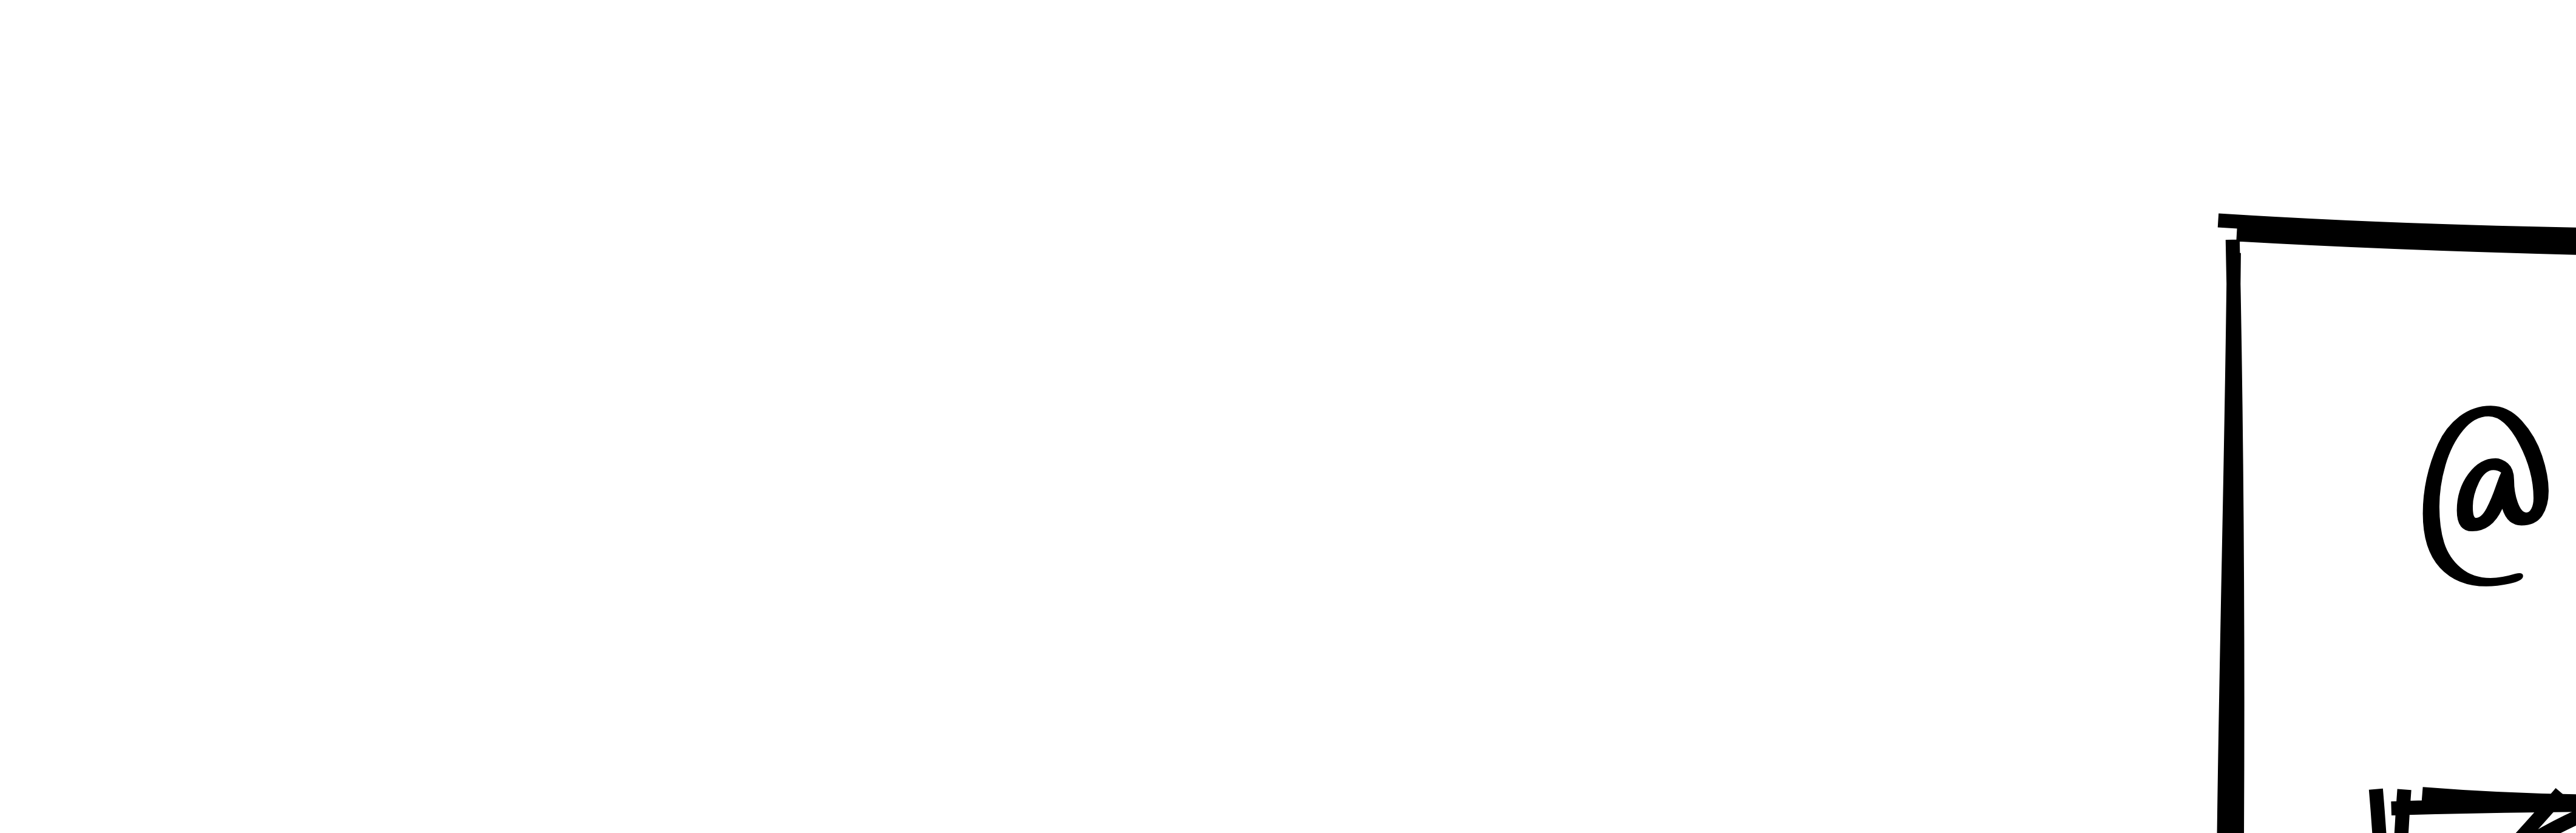
\includegraphics[width=\textwidth]{assets/forking_worker.png}
\end{frame}
\begin{frame}{Reusing event-loops}
    SCHEMA
\end{frame}
\begin{frame}{"Virtualizing" Netty event-loops}
    SCHEMA
\end{frame}
\begin{frame}{Deadlock: roles of the event-loop}
    \begin{enumerate}
        \item event-loop for the entire non-blocking inner-workings of the framework, 
        \item event-loop for the non-blocking endpoint handlers,
        \item work as a carrier thread for virtual threads
    \end{enumerate}
\end{frame}
\begin{frame}{Deadlock situation}
    SCHEMA    
\end{frame}
\begin{frame}{Deadlock: sharing locks}
    \begin{block}{Conclusion}
        The event-loop can't reuse locks \emph{as a carrier}
    \end{block}
\end{frame}


\section{Goals of the experiment}
\begin{frame}{Goals}
    \begin{itemize}
        \item Measure how performance of the application is affected by 
        \item second goal 
    \end{itemize}
\end{frame}
\begin{frame}{Hypothesis}
    \begin{block}{Hypothesis}
        Quarkus-virtual-threads should perform better than Quarkus-blocking but not as well as Quarkus-reactive
    \end{block}
\end{frame}

\section{Experimental protocol}
\begin{frame}{Elements of the experiment}
    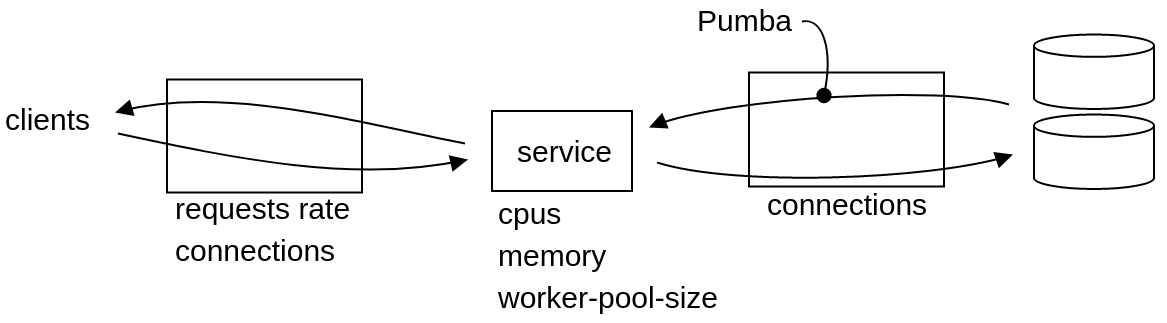
\includegraphics[width=\textwidth]{assets/exp.png}
\end{frame}

\section{Results}
\begin{frame}{Results without delay}
    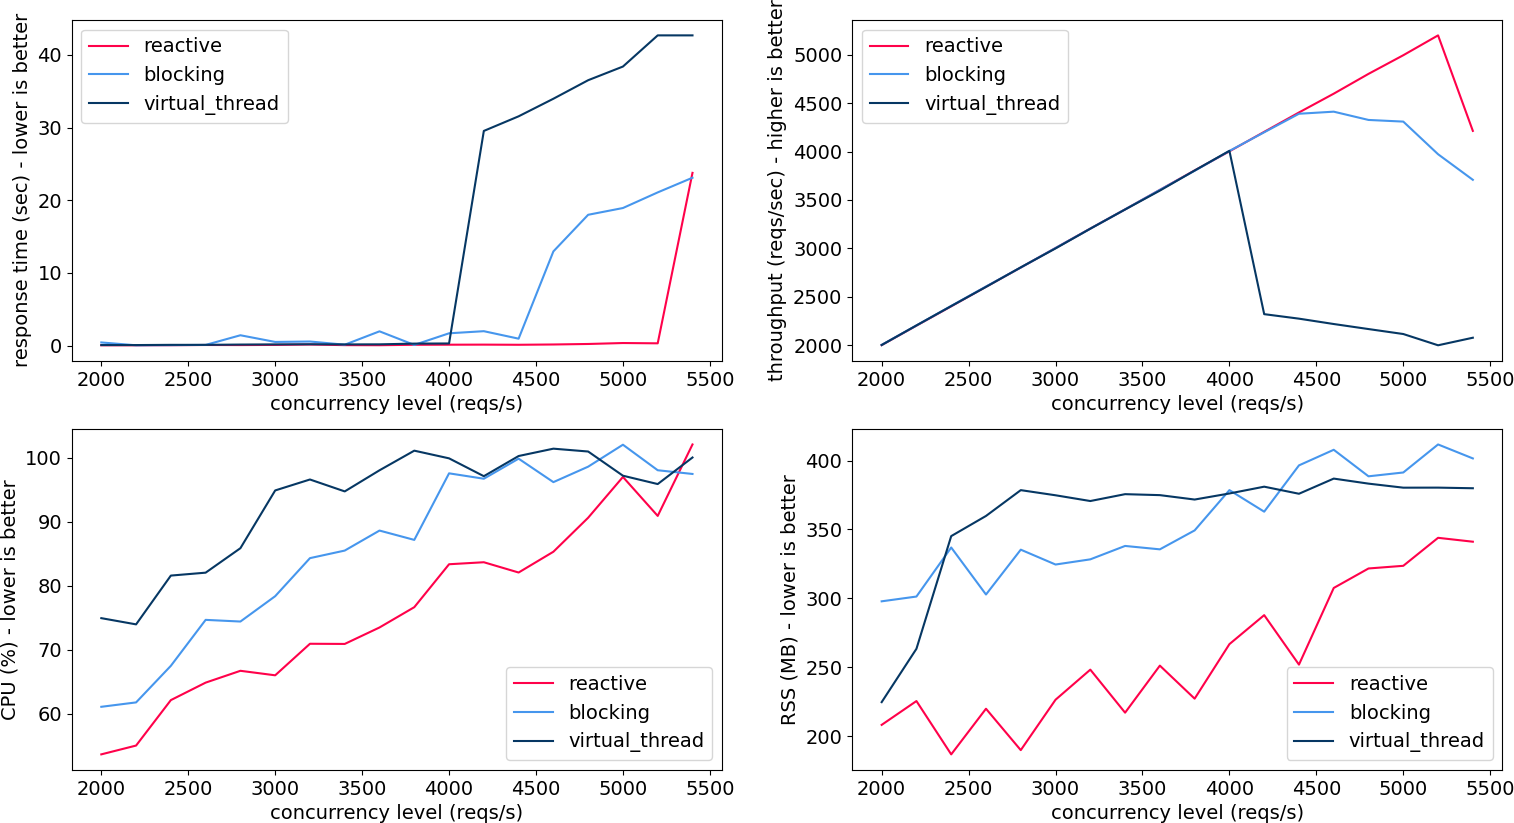
\includegraphics[width=\textwidth]{assets/nano_baseline_19.0.1.png}
\end{frame}
\begin{frame}{Results with 200ms delay}
    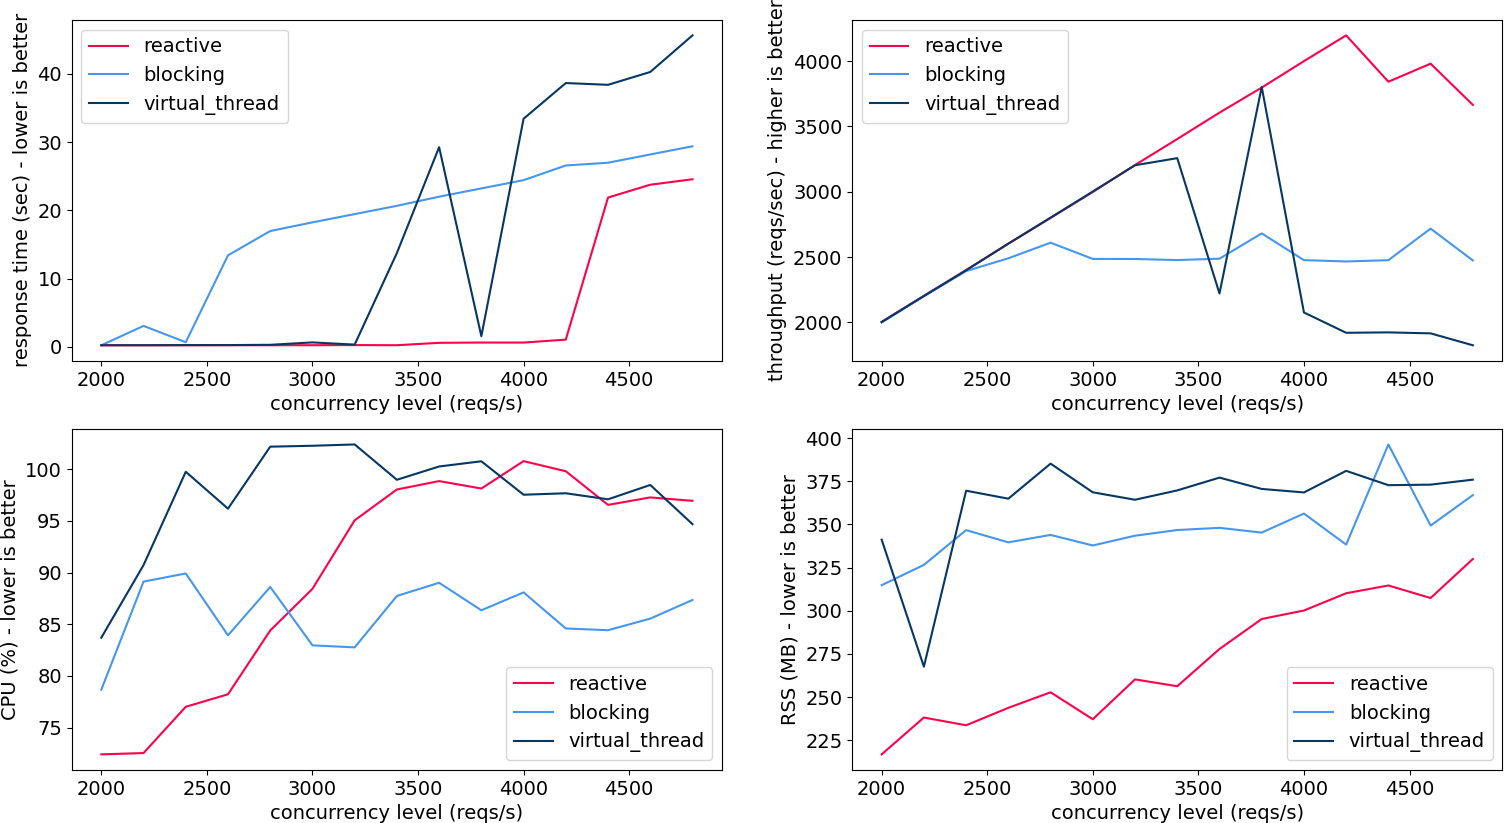
\includegraphics[width=\textwidth]{assets/nano_200_19.0.1.png}
\end{frame}
\begin{frame}{Conclusions}
    \begin{tabular}{l | c}
        performance &  Quarkus-blocking < Quarkus-virtual-threads < Quarkus-reactive \\
        \hline
        resource efficiency & x\\
    \end{tabular}
\end{frame}

\end{document}